\documentclass[11pt,a4paper,oneside]{report}

\usepackage[margin=1in]{geometry}
\usepackage[T1]{fontenc}
\usepackage{lmodern}
\usepackage{listings}
\usepackage{xcolor}
\usepackage{booktabs}
\usepackage{enumitem}
\usepackage{graphicx}
\usepackage{tikz}
\usetikzlibrary{arrows.meta,positioning,shapes.geometric,fit,calc}
\usepackage{amsmath}
\usepackage{microtype}
\usepackage[hidelinks]{hyperref}

\definecolor{codebg}{gray}{0.96}
\definecolor{codekw}{RGB}{0,90,160}
\definecolor{codecm}{RGB}{100,110,100}
\definecolor{figedge}{RGB}{60,60,60}

% Defined explicitly rather than relying on listings' built-in Rust support,
% which is absent from older distributions and errors out when requested.
\lstdefinelanguage{Rust}{
  keywords={as,async,await,break,const,continue,crate,dyn,else,enum,extern,
    false,fn,for,if,impl,in,let,loop,match,mod,move,mut,pub,ref,return,self,
    Self,static,struct,super,trait,true,type,unsafe,use,where,while},
  sensitive=true,
  morecomment=[l]{//},
  morecomment=[s]{/*}{*/},
  morestring=[b]",
}

\lstdefinestyle{rust}{
  language=Rust,
  backgroundcolor=\color{codebg},
  basicstyle=\ttfamily\small,
  keywordstyle=\color{codekw}\bfseries,
  commentstyle=\color{codecm}\itshape,
  breaklines=true,
  frame=none,
  xleftmargin=1em,
  framexleftmargin=1em,
  showstringspaces=false,
  captionpos=b
}
\lstset{style=rust}

% Deliberately takes no argument: the braces at each call site become an
% ordinary group, which keeps \verb usable inside the note text.
\newcommand{\note}{\par\smallskip\noindent\textit{Why it matters:} }
% Plain text (not \textsc): bold+small-caps is unavailable in Latin Modern.
\newcommand{\horizon}{Horizon}

\title{Mapping Free Functions without Compilation:\\[0.35em]
  \large A Vertical Account of the \horizon{} Function Map}
\author{}
\date{26 July 2026}

\begin{document}

\pagenumbering{roman}
\maketitle

\begin{abstract}
\horizon{} constructs a \emph{function map} of a Rust repository: a navigable
containment tree from repository through crates, folders, and files down to
free functions, each carrying an ordered sequence of outgoing call sites.
Each site resolves to exactly one definition, records a first-class
\texttt{Conflict} naming every candidate, or records \texttt{Unresolved}.
Recognised but out-of-scope call forms---external crates, methods,
\texttt{impl} items, constructors, associated functions---are dropped from the
tree entirely rather than mislabelled.

This report explains the system as a single continuous argument rather than as
a catalogue of source files. It follows the transformation of source text into
a map in the order the pipeline develops it: the problem that motivates a
structural, compile-free analyser; the choice of parser; the data model that
makes never-guessing representable; declaration-driven module discovery;
fact extraction from concrete syntax; name resolution with rustc-aligned
precedence; cross-crate reachability behind a dependency gate; deliberate
exclusions; allowlisted macro recovery; and finally the measurement regime
that distinguishes confident wrong edges from honest incompleteness.
Evaluation on unfamiliar repositories shows a bimodal usefulness result:
free-function pipelines yield informative maps, while method-centric and
definition-body macro architectures remain thin by design.

The organising principle throughout is that \textbf{the tool never guesses}.
That principle is not a slogan appended after the fact; it is the constraint
from which the \texttt{Conflict} node, the drop counters, the visibility
asymmetry, and the macro allowlists all follow.
\end{abstract}

\tableofcontents
\clearpage
\pagenumbering{arabic}

%==============================================================================
\chapter{The Problem}
\label{ch:problem}

\section{What a function map is for}

Software engineers routinely need a static picture of \emph{who calls whom}
across a real codebase: not a single file's outline, but a repository-scale
graph that remains navigable when the project is a Cargo workspace with path
dependencies, mid-edit files, and ambiguous imports. Indexing formats such as
SCIP and LSIF~\cite{scip,lsif} already answer a related question for
language servers and code hosts. They do so by invoking a full semantic
analysis---typically rust-analyzer's type-aware index---and they produce a
dense symbol table that includes methods, associated items, and cross-crate
references into the standard library.

\horizon{} answers a narrower question with a stricter honesty constraint.
It asks only for the free-function call structure of a Rust repository, and
it insists that every edge it draws be justified by name lookup that the
language itself would accept as decisive. Where the language refuses to pick
a winner, the map must refuse as well. Where a call form is recognised but
outside the free-function universe, the map must omit it rather than invent a
label that looks like a resolution failure.

The containment spine is:

\begin{center}
\texttt{Repository $\rightarrow$ Crate $\rightarrow$ Folder $\rightarrow$ File $\rightarrow$ Function}
\end{center}

Each free function carries its outgoing call sites in source order. Each call
site terminates in a \texttt{CallTarget}: a resolved reference to one
canonical function, a conflict naming several, or an unresolved marker. The
JSON contract that emits this structure is documented separately; this report
concerns the reasoning that makes the structure necessary.

\section{Why heuristics fail}

An earlier generation of the same project attempted to recover call structure
with lighter machinery---directory globs for ``source files,'' string-shaped
path matching, and when ambiguity arose, a ``likely'' edge labelled with a
confidence tag. The fixture corpus preserves the anti-example. Against a crate
that rustc rejects with error \texttt{E0659} (two glob imports supplying the
same name), the abandoned spike resolver emitted:

\begin{lstlisting}[language={}]
app.rs::run  ->  shapes.rs::get   [Likely, glob import]
\end{lstlisting}

That line is worse than silence. It asserts a unique callee where the
compiler asserts that no unique callee exists. Coverage metrics that count
``resolved'' edges would reward the guess; a consumer navigating the map would
follow a fabricated edge. The product rule that replaced this behaviour is
absolute: when two globs offer the same name and no local definition or
explicit import breaks the tie, the only correct emission is a
\texttt{Conflict} naming both candidates.

Regex and ad-hoc path splitting fail for a second, independent reason. Rust's
module system is declaration-driven. A file that sits on disk beside
\texttt{lib.rs} is not part of the crate unless a \texttt{mod} declaration
names it. Conversely, an inline module contributes a path segment with no
file of its own, and a \texttt{\#[path]} attribute can bind a tidy module name
to an arbitrarily renamed file. Directory listing invents modules the compiler
never sees and misses modules the compiler does.

\section{Why parse without compiling}

A natural response to the failure of heuristics is to demand a compiling
project: run \texttt{cargo check}, or ask rust-analyzer for unresolved
references, and map only what the toolchain accepts. That frame was considered
and rejected.

The cost of a compile gate is not merely latency. It reintroduces a toolchain
dependency for every analysis, refuses mid-edit repositories (precisely when a
navigable map is most useful), and throws away the error tolerance that
motivates choosing an industrial concrete-syntax parser in the first place.
Of the diagnostic classes that arise while exercising the rules this system
encodes---missing modules, private items, ambiguous globs, type mismatches---
almost all parse perfectly and fail later. Syntactic validity and
compilability are nearly orthogonal.

The replacement decision is: \textbf{build the tree always}. Problems become
visible as first-class map outcomes---\texttt{Conflict}, \texttt{Unresolved},
or a summary counter for a deliberate drop---rather than as a refused run.
Cargo remains in the pipeline, but only for crate discovery
(\texttt{cargo metadata --no-deps --offline}), which is a different job from
compilation.

\section{What this buys and what it costs}

Compile-free structural analysis buys three things that a SCIP-style index
does not simultaneously provide at the same cost: operation on non-compiling
trees; a deliberately small free-function universe that a frontend can render
without understanding Rust; and an explicit representation of ambiguity that
most semantic indexes collapse into ``unresolved reference'' or silently
prefer one candidate.

It costs nearly everything that requires types. Methods
(\texttt{x.foo()}), associated functions (\texttt{Type::name}), and trait
resolution are permanently out of scope---not deferred phases of this tool,
but a different product. Indirect calls through function pointers and
closures require dataflow. Macro-expanded module trees that live only inside
\texttt{macro\_rules!} definition bodies remain closed. The evaluation chapter
will show that these costs are not theoretical: on method-heavy repositories
the map is thin by construction, even when it is correct on every free
function it does index.

The remainder of this report develops the system that lives inside those
constraints. Each chapter picks up where the last left off, following source
text through discovery, parsing, extraction, resolution, and measurement
until the shape of the design is explained rather than merely described.

%==============================================================================
\chapter{Design Axioms}
\label{ch:axioms}

Before any pipeline stage is examined, four axioms must be stated. They are
the load-bearing decisions; later chapters are consequences.

\section{Never guess}

A call site in the indexed universe terminates in exactly one of three
outcomes:

\begin{enumerate}[nosep]
  \item \textbf{Resolved} --- name lookup found exactly one free-function
    definition. The edge holds a reference (\texttt{FunctionId}) to that
    canonical node.
  \item \textbf{Conflict} --- name lookup found two or more plausible
    definitions and the language does not allow picking one. The edge holds
    every candidate and a reason.
  \item \textbf{Unresolved} --- this is a free-function-shaped call, but no
    indexed definition matches. There are not several alternatives; there is
    no callee.
\end{enumerate}

\texttt{Conflict} is not an error channel. It is the concrete expression of
the never-guess principle: the map preserves the information that the language
itself treats as decisive refusal. Collapsing conflict into unresolved would
erase the distinction between ``many answers'' and ``no answer.'' Picking a
``likely'' winner would reintroduce the spike's false edge.

\section{The indexed universe}

The never-silently-missing rule applies \emph{within} the free-function
universe the tool indexes. It does not require every syntactic
\texttt{CallExpr} to appear as a site. External-crate calls, enum-variant and
tuple-struct constructors, and associated functions on types are recognised
and \textbf{dropped}: absent from the tree, tallied under dedicated summary
counters (\texttt{external\_dropped}, \texttt{constructor\_dropped},
\texttt{associated\_dropped}). Recording them as \texttt{Unresolved} would
mis-diagnose a type or an external crate as a missing free function---a
different and worse failure mode than omission.

This is the intellectual centre of the design. Completeness means: nothing
in-scope is silently missing. It does not mean: every parenthesis-shaped
construct is forced into the graph.

\section{Free functions only, permanently}

Methods and \texttt{impl}/\texttt{trait} items are permanently out of scope
for declarations and for call sites. Associated functions share that
exclusion. The cost is large: of \horizon{}'s own roughly 1{,}394 call sites
at measurement time, about 1{,}053 were method calls. Resolving them needs
type inference, not name lookup. A future type-aware product would be a
separate system, not an incremental extension of this map.

\section{Batch, always rebuild}

The tool is a single-shot batch analyser. There is no on-disk cache, no file
watcher, and no incremental state. Live updating while typing is a non-goal.
The host product's policy for when to rebuild remains open; the tool itself
answers one path with one map.

%==============================================================================
\chapter{Selecting a Parser}
\label{ch:parser}

\section{The criteria}

Three families of Rust parsers were available:

\begin{description}[style=nextline,leftmargin=1em]
  \item[\texttt{syn}] The almost-universal choice for procedural macros.
    It produces a tidy abstract syntax tree optimised for code generation.
    It discards comments and refuses to parse broken input.
  \item[\texttt{tree-sitter-rust}] An incremental, error-tolerant parser
    used widely in editors. It preserves a concrete tree and recovers from
    errors, but its Rust grammar and comment handling are a separate
    ecosystem from rust-analyzer's own understanding of the language.
  \item[\texttt{ra\_ap\_syntax}] rust-analyzer's syntax crate. It builds a
    lossless concrete syntax tree (CST), preserves comments and punctuation,
    parses incrementally, and yields a usable tree for incomplete input.
\end{description}

The criteria that decided the matter were exactly the capabilities the
compile-gate rejection had preserved as requirements: \textbf{error
tolerance} (mid-edit code must map), \textbf{comment preservation} (doc
comments are first-class map nodes), and a tree shape close enough to
rust-analyzer's own that later oracle comparisons against LSIF would not
fight an alien grammar.

\section{Concrete versus abstract trees}

An abstract syntax tree elides punctuation and trivia in favour of the
constructs a compiler's later passes need. A concrete syntax tree retains the
source's shape: attributes, doc comments, and token-tree interiors of macro
calls remain addressable. For a function map that must attach documentation
to the items it documents, and that must later open selected macro token
trees for recovery, the CST is not an implementation detail---it is the
substrate.

\texttt{syn}'s refusal to parse broken code would have made the ``build
always'' decision incoherent. Choosing \texttt{ra\_ap\_syntax} and then
gating on \texttt{cargo check} would have thrown away the principal reason
for the choice. The two decisions reinforce each other.

\section{What the wrapper does}

The parse stage in \horizon{} is deliberately thin. It accepts source text
and the edition string reported by cargo metadata, selects the corresponding
\texttt{ra\_ap\_syntax::Edition} (falling back to the crate's current edition
on unknown strings), and returns \texttt{SourceFile::parse(...).tree()}.
Parse errors are ignored at this boundary: they live on the \texttt{Parse}
value, and the tree is used regardless. Measured extraction throughput on an
early spike was roughly 1.2\,MB/s single-core; later scale validation on dense
trees lands around 0.8--1.1\,MB/s of analysed source for the full pipeline.

\section{What parsing does not decide}

A CST tells the extractor what was written. It does not resolve names, enforce
privacy, expand macros, or decide which \texttt{\#[cfg]} arm is live. Those
questions belong to later stages, and several of them are answered with the
never-guess rule rather than with a build configuration. The parser's job ends
when a tree exists.

%==============================================================================
\chapter{The Function Map as a Data Structure}
\label{ch:model}

\section{Containment is a tree}

Containment does not cycle. The emitted hierarchy is therefore a tree:

\begin{figure}[ht]
\centering
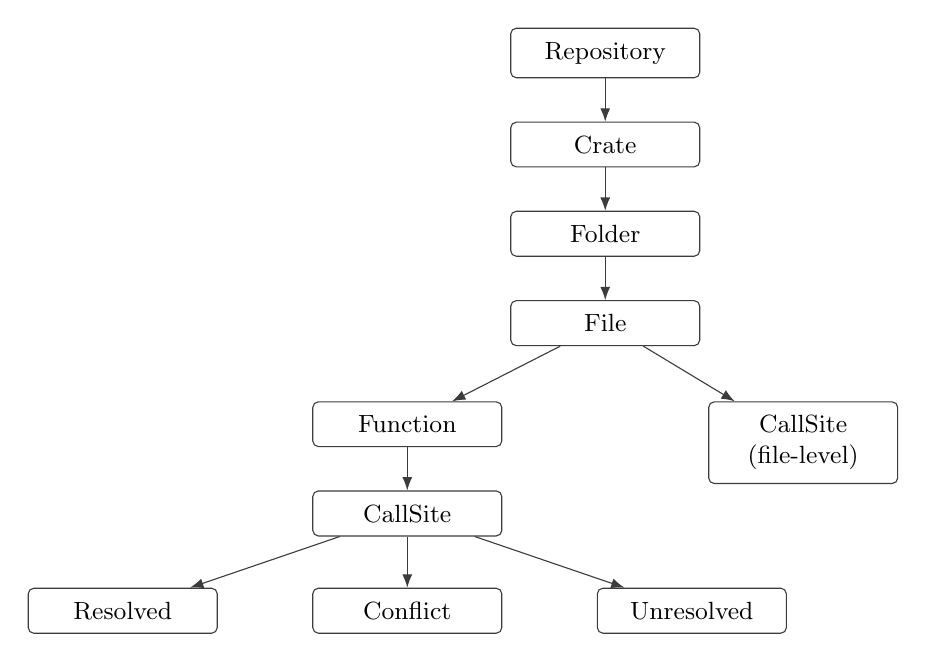
\begin{tikzpicture}[
  font=\small,
  box/.style={draw=figedge, rounded corners=2pt, align=center,
    inner sep=5pt, minimum width=2.4cm},
  arr/.style={-{Latex}, figedge}]
  \node[box] (repo) {Repository};
  \node[box, below=0.55cm of repo] (crate) {Crate};
  \node[box, below=0.55cm of crate] (folder) {Folder};
  \node[box, below=0.55cm of folder] (file) {File};
  \node[box, below left=0.7cm and 0.1cm of file] (fn) {Function};
  \node[box, below right=0.7cm and 0.1cm of file] (fcall) {CallSite\\(file-level)};
  \node[box, below=0.55cm of fn] (call) {CallSite};
  \node[box, below left=0.65cm and 1.2cm of call] (res) {Resolved};
  \node[box, below=0.65cm of call] (conf) {Conflict};
  \node[box, below right=0.65cm and 1.2cm of call] (unr) {Unresolved};
  \draw[arr] (repo) -- (crate);
  \draw[arr] (crate) -- (folder);
  \draw[arr] (folder) -- (file);
  \draw[arr] (file) -- (fn);
  \draw[arr] (file) -- (fcall);
  \draw[arr] (fn) -- (call);
  \draw[arr] (call) -- (res);
  \draw[arr] (call) -- (conf);
  \draw[arr] (call) -- (unr);
\end{tikzpicture}
\caption{Containment hierarchy and call-target terminals. Folders nest;
  modules are not spine nodes. Doc-comment leaves are omitted for clarity.}
\label{fig:hierarchy}
\end{figure}

Crates sit above folders because crates do not nest like directories. A
repository may hold independent packages with no root manifest; a package's
library and its \texttt{src/bin/*.rs} binaries are separate compilation units
that share a directory. The path text \texttt{crate::...} means different
things in different crates. Treating the filesystem as the spine would
collapse those distinctions.

Modules are intentionally absent from the spine. The working assumption that
``module equals file'' is false in four ways the compiler exhibits: ordinary
\texttt{mod} files, inline modules with no file, undeclared files that never
compile, and \texttt{\#[path]} renames. Two functions of the same name at
different module depths in one file are distinguished by their recorded module
paths and by their \texttt{FunctionId}s, not by inventing module nodes the
folder tree cannot host.

\section{References, not copies}

A resolved call site stores a \texttt{FunctionId}---a reference to the one
canonical \texttt{Function} object---never an embedded copy of that function.
The same holds for conflict candidates. This is what makes recursion
tractable: \texttt{countdown} calling \texttt{countdown} is a pointer back to
the same node. A function called from thirty places exists once and is
referenced thirty times. Expanding resolved targets by value would loop
forever or explode the JSON.

Conflicts hold function references rather than file references because
\texttt{\#[cfg(unix)] fn open()} and \texttt{\#[cfg(windows)] fn open()} can
sit in the same file. Storing files would collapse them. Every function knows
its parent file through containment, so the file list remains derivable.

\section{Function identity}
\label{sec:function-id}

\texttt{FunctionId} uniquely names one definition across the repository:

\begin{center}
\begin{tabular}{@{}ll@{}}
\toprule
Library & \texttt{\{rustc\_name\}::\{module\_path\}} \\
Binary  & \texttt{\{rustc\_name\}[bin]::\{module\_path\}} \\
Collision & append \texttt{\#L\{line\}} to every collider \\
\bottomrule
\end{tabular}
\end{center}

The \texttt{[bin]} marker uses characters illegal in Rust identifiers and
Cargo package names, so it cannot be confused with a real crate. An earlier
approach that rewrote binaries to \texttt{horizon\_bin} was rejected: that
string looks like a package that could actually exist. The crate's
\texttt{rustc\_name} field always stores the real cargo target name; only the
id prefix carries the disambiguator.

Internally, module paths keep a leading \texttt{crate} segment
(\texttt{crate::shapes::get}). The id substitutes the crate key for that
segment (\texttt{text\_engine::shapes::get}). The leading segment is replaced,
not prepended, so the id does not name the crate twice.

The line suffix is appended \textbf{only} when two or more definitions share
the same crate-key-plus-module path. Unique paths stay free of line numbers,
so ordinary ids do not churn when unrelated edits shift lines. Ids are
assigned after all definitions in a crate are collected, so collisions are
detected crate-wide. Because every id is prefixed by a compilation-unit key,
definitions in different crates---including a package's same-named lib and
bin---cannot collide inside one repository map.

\section{Call sites on files}

Calls that sit outside any free function---typically a \texttt{const} or
\texttt{static} initialiser invoking a \texttt{const fn}---attach to the
owning \texttt{File}, reusing the same \texttt{CallSite} type and the same
resolver. Inventing a synthetic pseudo-function was rejected: it would pollute
the function list and invent an identity the source does not have. Calls
inside \texttt{impl}/\texttt{trait} bodies are not swept into the file-level
list; methods remain out of scope.

\section{Summary counters}

The repository carries a \texttt{MapSummary}: counts of conflicts, unresolved
sites, and the three drop categories. Resolved edges are not counted there.
The counters exist so map health is visible without walking the tree, and so
``excluded by design'' is never conflated with ``could not resolve.''

%==============================================================================
\chapter{Discovering Compilation Units}
\label{ch:discover}

\section{Cargo metadata as a read-only oracle}

Crate discovery runs
\texttt{cargo metadata --no-deps --format-version 1 --offline} per manifest,
retrying without \texttt{--offline} if the lockfile or index is unavailable,
but never dropping \texttt{--no-deps}. Full metadata can create or update
\texttt{Cargo.lock} in a repository the tool does not own---forbidden for a
read-only analyser. The invocation performs no compilation; on \horizon{}
itself it was measured at a few hundred milliseconds.

\texttt{--no-deps} lists only workspace members. Path dependencies outside
that set are found by recursing into each dependency's \texttt{path}
directory and running metadata there. Registry and git dependencies are never
walked.

\section{One node per compilation unit}

Discovery emits one \texttt{Crate} node per mapped target, not per package.
Library-like kinds (\texttt{lib}, \texttt{rlib}, \texttt{dylib},
\texttt{cdylib}, \texttt{staticlib}, \texttt{proc-macro}) and binaries are
included. Examples, integration tests, benches, and \texttt{build.rs} are
deliberately excluded: they are secondary surfaces that inflate maps and hit
the \texttt{[dev-dependencies]} blind spot.

\texttt{proc-macro} is included explicitly because cargo metadata reports it
as its own kind. Omitting it silently dropped crates such as
\texttt{serde\_derive}---ordinary free functions inside procedural-macro
crates would vanish from the map.

Same-package binaries receive an implicit path dependency on their package
library, matching Cargo. Manifest rename aliases
(\texttt{alias = \{ package = "real-name", path = "..." \}}) are recorded:
the import rustc name (alias when present) is what code and the dependency
gate use; the package name identifies the path edge.

\section{Fixtures must not pollute self-maps}

When analysing the \horizon{} repository itself, discovery skips
\texttt{tests/fixtures/**}. Those crates are deliberately broken or ambiguous
specimens. Mapping them as ordinary source would corrupt every self-test.
Nested fixture packages also declare an empty \texttt{[workspace]} table so
Cargo does not claim them when checked via \texttt{--manifest-path}.

\section{Consequence for resolution}

Once crates are spine nodes with declared dependency lists, the dependency
graph becomes a hard constraint on resolution. If crate A does not depend on
crate B, no name in A may resolve into B---a far more reliable filter than
name uniqueness across a repository. Chapter~\ref{ch:cross-crate} returns to
this gate.

%==============================================================================
\chapter{Following the Module Tree}
\label{ch:modules}

\section{Declaration-driven discovery}

From each target's root file, the walker follows \texttt{mod} declarations
transitively. It never globs the directory. The four compiler-verified
divergences between modules and files are the proof that globbing is wrong:

\begin{table}[ht]
\centering
\begin{tabular}{@{}lll@{}}
\toprule
\textbf{Case} & \textbf{Module} & \textbf{File} \\
\midrule
Ordinary       & \texttt{text}       & \texttt{text.rs} \\
Inline module  & \texttt{text::case} & none --- inside \texttt{text.rs} \\
Undeclared     & none                & \texttt{orphan.rs} --- never compiled \\
\texttt{\#[path]} & \texttt{tidy\_name} & \texttt{renamed\_on\_disk.rs} \\
Crate root     & the root itself     & \texttt{lib.rs} --- no path segment \\
\bottomrule
\end{tabular}
\caption{Module/file divergences that forbid directory-glob discovery.}
\label{tab:mod-file}
\end{table}

The fixture \texttt{phase2-modules} places garbage in an undeclared
\texttt{orphan.rs}:

\begin{lstlisting}
//! Undeclared garbage --- must never appear in the function map.
this is not rust!!!
fn should_not_be_indexed() {
    nonsense();
}
\end{lstlisting}

A file containing pure syntactic garbage compiles fine as long as no
\texttt{mod} declaration names it. Globbing would index it; the declaration
walk never opens it.

The \texttt{path-dependency} fixture binds a tidy name to a renamed file:

\begin{lstlisting}
#[path = "renamed_on_disk.rs"]
pub mod tidy_name;
\end{lstlisting}

The module path is \texttt{crate::tidy\_name}, not the on-disk stem. Calls and
ids must use the module name the language sees.

\section{Inline modules and nesting}

An inline \texttt{mod name \{ ... \}} extends the module path and visibility
tables but creates no \texttt{File} node. A subtle consequence, verified in
fixtures: a file \texttt{selfdecl.rs} declared as \texttt{mod selfdecl} that
itself contains \texttt{pub mod selfdecl \{ ... \}} \emph{nests} rather than
merging. The inner function's path is
\texttt{crate::selfdecl::selfdecl::inner\_fn}.

\section{First declaration wins}

Repeated declarations of the same module path terminate that branch: the first
declaration wins. The practical limitation is cfg-twinned modules with
different \texttt{\#[path]} targets---only the first file is kept. One module
path maps to one file. Cycles are handled by the same seen-set. Missing module
files are reported and skipped without panicking.

\section{Item-macro module recovery (preview)}

\texttt{mod} declarations hidden inside allowlisted item macros
(\texttt{cfg\_if!}, Tokio-style names starting \texttt{cfg\_}) are recovered
by re-parsing the invocation token tree, depth-bounded at 8, with all
\texttt{cfg\_if!} branches unioned. The tool does not choose a build
configuration---the same spirit as keeping \texttt{\#[cfg]}-duplicated
functions. Chapter~\ref{ch:macros} develops the full recovery argument,
including why serde's \texttt{crate\_root!()} pattern stays closed.

\section{Folders from walked files only}

After extraction and resolution, each compilation unit builds its folder tree
from the files the module walk found, independently of every other unit. A
library and its \texttt{src/bin/} binaries sharing a directory do not
interleave files. Undeclared neighbours never appear.

%==============================================================================
\chapter{Extracting Facts from Concrete Syntax}
\label{ch:extract}

\section{What extraction collects}

For each discovered file, at the crate's real edition, extraction walks the
CST and collects:

\begin{itemize}[nosep]
  \item free-function definitions (with visibility), including nested free
    functions;
  \item local type names---structs, enums with variants, traits, type
    aliases---used later to classify constructors and associated functions;
  \item the import table from \texttt{use}/\texttt{pub use} trees and
    \texttt{extern crate} renames, flattened from the AST rather than by
    string splitting;
  \item path-form call sites, owned either by an enclosing free function or
    by the file;
  \item doc comments: outer forms on functions, inner forms on files.
\end{itemize}

Methods and anything inside \texttt{impl}/\texttt{trait} items are skipped at
extraction time. They never become pending call sites, so they cannot be
mislabelled as unresolved free functions later.

\section{Import tables}

Supported forms include plain paths, brace lists, nested braces, aliases,
\texttt{self} in a brace list (binds the module), globs, re-exports, renamed
re-exports, glob re-exports, relative roots (\texttt{self::}, \texttt{super::},
\texttt{crate::}), and \texttt{pub extern crate dep as name}. Discard imports
(\texttt{as \_}) contribute no binding. External roots such as
\texttt{std::fs} are recorded as external so later calls through the binding
can be dropped rather than unresolved.

A known limitation is recorded rather than hidden: a \texttt{use} inside a
function body is attributed to the enclosing module with
\texttt{scope\_widened = true}. Resolution therefore treats it as module-wide,
which is wider than rustc. The flag exists so the limitation is never silent;
as of this writing the resolver does not special-case the flag---the widening
is unconditional for such imports.

\section{Doc comments}

\texttt{ra\_ap\_syntax} keeps outer docs and attributes as children of the
item, so \texttt{///} docs followed by \texttt{\#[inline]} still attach to the
function. Consecutive pieces of the same kind on one owner are joined with
newlines into a single \texttt{DocComment}, matching rustdoc's one-logical-
comment rule. Ordinary \texttt{//} comments never appear. Whitespace stripping
removes exactly one leading ASCII space after the marker and preserves further
indentation for fenced code blocks.

\section{Pass ordering}

Every discovered crate is extracted before any crate is resolved. Cross-crate
edges need callees to exist. Function ids are assigned crate-wide after each
crate's definitions are known, then pending call owners are remapped to those
ids. The shared \texttt{pipeline} module constructs the extract $\rightarrow$
resolve-index path used by both the CLI and the correctness harness, so
measurements cannot drift from production.

%==============================================================================
\chapter{Name Resolution as a Calculus}
\label{ch:resolve}

\section{The intellectual centre: Conflict}

Consider the minimal fixture that exists solely to trigger rustc
\texttt{E0659}:

\begin{lstlisting}
use crate::shapes::*;
use crate::text::*;

pub fn run() -> usize {
    get(3)
}
\end{lstlisting}

Both sibling modules define \texttt{get}. There is no explicit import and no
local definition. rustc rejects the crate. The abandoned spike guessed
\texttt{shapes::get}. \horizon{} emits a \texttt{Conflict} naming
\texttt{glob\_ambiguity::shapes::get} and \texttt{glob\_ambiguity::text::get}.

The twin fixture adds one line:

\begin{lstlisting}
use crate::text::get;
\end{lstlisting}

rustc accepts the crate; the explicit import outranks the globs;
\texttt{get(3)} resolves uniquely to \texttt{text::get}. The map must emit a
single resolved edge---not a conflict, and not a coin-flip.

These two crates are the clearest statement of the design. Ambiguity is not a
degraded form of success. It is a different terminal.

\section{Precedence}
\label{sec:precedence}

Within-crate unqualified lookup follows rustc, verified against the glob
fixtures:

\begin{figure}[ht]
\centering
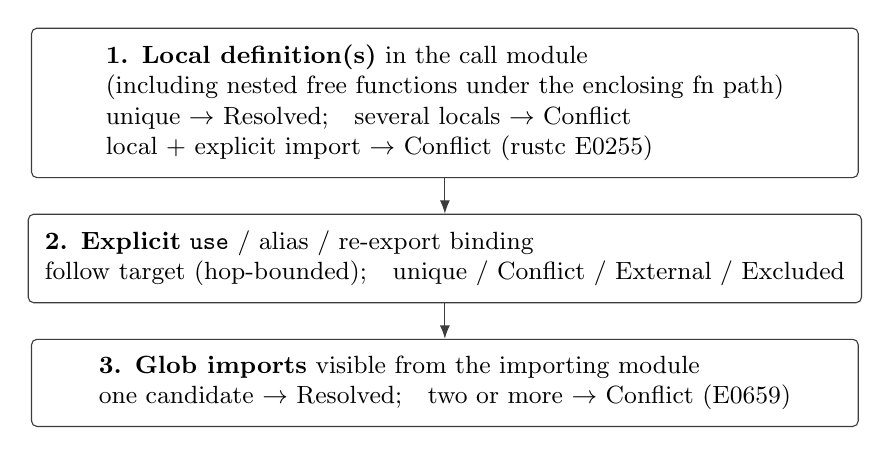
\begin{tikzpicture}[
  font=\small,
  stage/.style={draw=figedge, rounded corners=2pt, align=left,
    inner sep=6pt, minimum width=10.5cm},
  arr/.style={-{Latex}, figedge}]
  \node[stage] (s1) {\textbf{1. Local definition(s)} in the call module\\
    (including nested free functions under the enclosing fn path)\\
    unique $\rightarrow$ Resolved;\quad several locals $\rightarrow$ Conflict\\
    local + explicit import $\rightarrow$ Conflict (rustc E0255)};
  \node[stage, below=0.45cm of s1] (s2)
    {\textbf{2. Explicit} \texttt{use} / alias / re-export binding\\
    follow target (hop-bounded);\quad unique / Conflict / External / Excluded};
  \node[stage, below=0.45cm of s2] (s3)
    {\textbf{3. Glob imports} visible from the importing module\\
    one candidate $\rightarrow$ Resolved;\quad two or more $\rightarrow$ Conflict (E0659)};
  \draw[arr] (s1) -- (s2);
  \draw[arr] (s2) -- (s3);
\end{tikzpicture}
\caption{Unqualified name-resolution precedence. The tool never picks a
  winner among equal-ranked candidates.}
\label{fig:precedence}
\end{figure}

Qualified paths navigate \texttt{crate::}, \texttt{self::}, \texttt{super::}
(including multi-\texttt{super}), then module segments and import bindings.
Facade re-exports are followed with a shared hop bound of 32
(\texttt{REEXPORT\_HOP\_LIMIT}). Exhausting the bound yields
\texttt{Unresolved}; the cross-crate entry path includes the limit in the
reason string so a re-export cycle cannot hang the tool.

\section{Visibility asymmetry}
\label{sec:visibility}

Three distinct policies apply. They look inconsistent until each is justified:

\begin{description}[style=nextline,leftmargin=1em]
  \item[Direct within-crate edges.] Visibility is \emph{not} filtered. A path
    the author wrote still appears even when rustc would emit \texttt{E0603}.
    Mid-edit code must stay mappable. The never-guess rule forbids picking
    among candidates; it does not require pretending a written call does not
    exist.
  \item[Glob candidate sets.] Visibility \emph{is} filtered. A glob only
    brings in names visible from the importing module through the globbed
    module. Including private items would manufacture \texttt{E0659} conflicts
    rustc would never report---false conflicts, the dual of false
    resolutions.
  \item[Cross-crate reachability.] Visibility \emph{is} enforced: a
    \texttt{pub} item behind an all-\texttt{pub} module chain, or a
    \texttt{pub} facade that exposes the item without naming private
    intermediates. \texttt{pub(crate)} stops at the crate boundary.
\end{description}

Keep the asymmetry deliberate. Within-crate direct edges map what the author
wrote. Cross-crate edges map what is actually nameable from outside. Glob
filtering protects the conflict predicate from pollution.

\section{Cfg twins}

\begin{lstlisting}
#[cfg(unix)]
fn open() {}

#[cfg(windows)]
fn open() {}
\end{lstlisting}

Both definitions appear in the syntax tree. Function ids receive
\texttt{\#L\{line\}} suffixes. A call to \texttt{open()} becomes a
\texttt{Conflict} naming every candidate. The tool does not choose a build
configuration. That is the never-guess outcome, not a silent pick---and on
real corpora it is a common, honest source of map noise.

\section{Unresolved is not a dustbin}

\texttt{Unresolved} means: this is a free-function call we genuinely could
not resolve. Typical causes include a typo, a name that exists only behind an
unopened macro, a path into a workspace sibling that is not a declared
dependency, or---on real corpora---test-only externals that discovery never
listed because \texttt{[dev-dependencies]} are omitted. It must not be used
for constructors, associated functions, or external crates. Those have their
own exits from the resolver.

%==============================================================================
\chapter{Crossing Crate Boundaries}
\label{ch:cross-crate}

\section{The dependency gate}

Crate A may resolve into crate B only when A declares B as a path dependency.
Workspace membership alone is not enough. The
\texttt{workspace-dep-gate} fixture places the same \texttt{pub fn shared} in
\texttt{dep\_a} and \texttt{dep\_b}; the consumer depends only on
\texttt{dep\_a}. Naming \texttt{dep\_b::shared} must remain
\texttt{Unresolved}---never a wrong edge into the undeclared sibling.

This gate is the payoff for elevating crates to spine nodes
(Chapter~\ref{ch:discover}). Name uniqueness across a repository is a weak
filter; the declared dependency graph is a hard one.

\section{Cross-crate visibility}

Once the gate opens, reachability still requires:

\begin{enumerate}[nosep]
  \item every \emph{named} module segment from the foreign crate root to be
    \texttt{pub};
  \item the target item itself to be \texttt{pub};
  \item or a \texttt{pub} facade that exposes the item under a public name,
    including \texttt{pub use private\_mod::item} (Rust-correct: the
    re-export name is public even when the module is not).
\end{enumerate}

\texttt{pub(crate) use} is invisible from outside. A path that names a
private foreign module (for example \texttt{text\_engine::secret::hidden})
remains unreachable even if the function inside is \texttt{pub}.

\section{Facade following}

Published Rust libraries conventionally present a flat crate-root API and
treat internal crates as private. Leaving facade paths unresolved was the
largest remaining resolution gap on multi-crate corpora. \horizon{} follows:

\begin{itemize}[nosep]
  \item \texttt{pub use eng::upper}
  \item renamed \texttt{pub use eng::tokenize as split}
  \item \texttt{pub use eng::*}
  \item \texttt{pub extern crate eng as name} (ripgrep-style barrels)
  \item multi-crate chains (facade $\rightarrow$ mid $\rightarrow$ leaf)
\end{itemize}

Following a hop into a third crate that the \emph{foreign} crate declares does
not require the consumer to declare that third crate. The consumer's
\emph{initial} entry still needs the dependency edge. Two foreign glob
re-exports offering the same name produce a \texttt{Conflict}, never a pick.
All re-export walks share the hop bound of 32.

Scale validation after facade following recovered ripgrep edges such as
\texttt{grep::cli::hostname} resolving to the defining function in
\texttt{grep\_cli}, and rust-analyzer barrel paths such as
\texttt{hir::db::file\_item\_tree} resolving into \texttt{hir\_def}. Hand
spot-checks of the newly resolved facade sample found no false positives.

\section{Consumer-side globs remain closed}

\texttt{use dep::*} in the \emph{calling} crate is not specially expanded.
Foreign crates' own \texttt{pub use dep::*} facades \emph{are} followed. The
distinction matches how published APIs are actually structured: the facade
author chooses the public surface; a consumer glob is a different, wider
request that would require importing another crate's entire public namespace
into the local conflict calculus.

%==============================================================================
\chapter{Deliberate Absences}
\label{ch:exclusions}

Each exclusion below is a design decision with a recorded cost, not a gap
waiting to be filled inside this tool.

\section{Methods and associated functions}

Method declarations and \texttt{x.foo()} call sites are permanently out of
scope. Associated functions (\texttt{Vec::new}, \texttt{Type::assoc}) share
the exclusion and are counted in \texttt{associated\_dropped}. Both are
\texttt{impl} items. Resolving them needs the type of the receiver or the
type segment, which is type inference. Even a future type-aware tool would
still face receivers behind generics and trait objects.

Classification of associated-function forms prefers collected type facts,
prelude names, and primitives; when facts are absent it falls back to a
strict UpperCamelCase heuristic (ASCII uppercase start, alphanumeric only,
at least one lowercase---not \texttt{ALL\_CAPS}). Segments that fail the
heuristic surface as \texttt{Unresolved} rather than silent drops. Modules
present in the module tree are navigated as modules regardless of
capitalisation; UpperCamelCase modules \emph{absent} from the tree can still
be mis-dropped---a documented residual risk.

\section{Constructors}

Enum variants and tuple-struct constructors are syntactically
\texttt{CallExpr} in \texttt{ra\_ap\_syntax} but construct a value rather than
invoke a free function. They are absent from the tree and counted in
\texttt{constructor\_dropped}. Recording \texttt{Ok(x)} as unresolved would
mis-diagnose a prelude constructor as a missing function.

\section{External calls}

Calls into \texttt{std}/\texttt{core}/\texttt{alloc}/\texttt{proc\_macro}, or
into a Cargo dependency whose kind is external, are deliberately dropped and
counted in \texttt{external\_dropped}. Path dependencies are not dropped by
this rule. Someone reading the never-silently-missing rule literally might
try to ``restore'' external calls as unresolved sites. Do not: external
callees are outside the indexed universe. A function whose body only calls
\texttt{std} appears as a childless leaf; that is intentional.

\section{Indirect calls and functions as values}

A call through a parameter or closure binding needs dataflow.
\texttt{apply(\&n, normalize)} records the call to \texttt{apply} but not the
reference to \texttt{normalize}. Both relationships are real and both are
absent; the second vanishes completely from the map.

\section{Secondary Cargo surfaces}

Examples, tests, benches, and \texttt{build.rs} are not discovered.
\texttt{[dev-dependencies]} are omitted from the dependency list used for
resolution. Scale validation shows the cost: test-only externals often surface
as \texttt{Unresolved} rather than \texttt{external\_dropped}. Including them
as external roots (not walked) remains an open product decision.

\section{SCIP as production indexer}

\texttt{rust-analyzer scip} produces a full semantic index with real name
resolution and type inference---measured at 73\,s / 2.1\,GB on ruff with
roughly 81\% of references resolved, including methods. The hand-built
approach resolves a smaller fraction of path-form calls with methods excluded.
The decision to build a custom free-function map anyway trades coverage for
compile-free operation, an explicit conflict terminal, doc comments as
first-class nodes, and independence from a rust-analyzer component in the
production path. LSIF from rust-analyzer is used only as a correctness oracle
on \horizon{} itself, not as the production indexer.

%==============================================================================
\chapter{Recovering What Macros Hide}
\label{ch:macros}

\section{Why token trees make calls invisible}

The parser leaves macro arguments as unstructured token trees. The call
\texttt{mean(v)} inside \texttt{format!("\{\}", mean(v))} is invisible to a
normal \texttt{CallExpr} walk. Measured on \horizon{}, this hid on the order
of tens of path-form calls against a few hundred visible ones---enough to
matter, not enough to justify opening every macro.

\section{Allowlist and reparse}

Recovery opens only an allowlist of std/core macros whose arguments are
expression positions: \texttt{format!}, \texttt{print!}/\texttt{println!}/
\texttt{eprint!}/\texttt{eprintln!}, \texttt{write!}/\texttt{writeln!},
\texttt{assert!} family, \texttt{debug\_assert*} family, \texttt{vec!},
\texttt{dbg!}, \texttt{panic!}, \texttt{unreachable!},
\texttt{unimplemented!}, \texttt{todo!}. For each, the token-tree interior is
re-parsed as Rust (parenthesised arguments become arguments of a synthetic
callee; brackets become an array literal) and path-form \texttt{CallExpr}s
are collected with ranges mapped back into the original file. Nested
allowlisted macros found after reparse are opened recursively, depth-bounded.
Recovered sites resolve through the normal path and set
\texttt{CallSite.from\_macro} (omitted from JSON when false).

A span-fidelity check requires the mapped byte range to match the original
token-tree text, rejecting reparse phantoms. Deduplication against ordinary
CST sites prevents double counting.

\section{Look-alikes that must stay closed}

The same token shape appears in places that are not calls:

\begin{lstlisting}
// Genuine calls hidden in token trees (must be recovered).
let _ = format!("{}", mean(v));
println!("{}", width_of(s));

// Traps --- must stay absent from the map.
let _ = matches!(Some(1), Some(_y));   // pattern, not a call
let _ = stringify!(helper());          // tokens, not evaluation
let _ = vec![Foo(1), Foo(2)];          // constructors
identity_call!(mean(v))                // macro_rules / user macro
\end{lstlisting}

\texttt{matches!}, \texttt{stringify!}, \texttt{concat!}, \texttt{include*!},
\texttt{cfg!}, \texttt{quote!}, \texttt{macro\_rules!} definition bodies,
attribute and derive token trees, and all user-defined macros stay opaque.
Prefer a miss over a fabricated edge. Tuple-struct constructors recovered
inside allowlisted macros still hit the classifier and are dropped as
constructors.

\section{Item-macro module recovery}

Item-pasting macros hide \texttt{mod} declarations the same way. The
allowlist is \texttt{cfg\_if!} and names starting with \texttt{cfg\_}
(Tokio-style \texttt{cfg\_fs!}, \ldots). All \texttt{cfg\_if!} branches are
unioned. Nested allowlisted macros open up to depth 8. Missing files on a
branch are skipped without panicking.

\textbf{Not recovered---serde \texttt{crate\_root!()}.} The real modules live
in a \texttt{macro\_rules!} \emph{definition} body; the invocation is an empty
\texttt{crate\_root!()}. Expanding definition bodies is a different and
riskier problem than re-parsing an invocation's tokens. Prefer a missing
subtree over a fabricated module tree. Scale validation confirms the
consequence: after proc-macro discovery, \texttt{serde\_derive} appears, but
serde's main library remains thin.

%==============================================================================
\chapter{Measuring Correctness}
\label{ch:correctness}

\section{Coverage is not correctness}

A confidently wrong \texttt{Resolved} edge is worse than an honest
\texttt{Conflict}. Coverage metrics that reward resolution rate incentivise
exactly the spike's ``likely'' behaviour. Correctness measurement therefore
asks a different question: among edges the tool claims to have resolved, how
often is that claim false?

\section{Three complementary oracles}

\begin{description}[style=nextline,leftmargin=1em]
  \item[Hand-annotated fixtures.] Primary standing check.
    \texttt{expected-edges.json} files encode required resolved targets,
    conflicts, unresolved sites, and required absences. They cover
    non-compiling crates that SCIP/LSIF cannot index.
  \item[Adversarial fixture.] Directly probes confident wrong edges: same
    name at several module depths, local-versus-glob, rename chains, cfg
    twins, module/function name collision, nested-inline shadowing.
  \item[rust-analyzer LSIF on \horizon{} itself.] Compiler-grade name
    resolution over real code, filtered to free-function monikers. SCIP is
    available but LSIF is JSON and needs no extra crate for comparison.
\end{description}

The harness never changes the resolver's answers; it only compares them. It
shares the extract $\rightarrow$ resolve-index pipeline with the CLI.

\section{Snapshot results and what they establish}

On the standing harness (26 July 2026 snapshot): 59 / 59 fixture oracle edges
passed with \textbf{zero false positives}; every required conflict stayed a
conflict; no case resolved to a guessed winner. On an atomically generated
self-map + LSIF pair: 411 resolved edges compared, 411 agreed with a
same-name free-function moniker, \textbf{zero false positives}, including a
separate cohort of 37 macro-recovered sites.

\section{What zero false positives does not establish}

Treat the result with proper scepticism.

\begin{enumerate}[nosep]
  \item Everything measured at LSIF grade is \horizon{}'s own small, clean
    source tree plus purpose-built fixtures. That is not evidence about large,
    messy corpora.
  \item Cross-crate precision beyond multi-crate fixtures lacks a foreign
    \texttt{FunctionId} LSIF filter; newly resolved facade edges on large
    corpora still need hand spot-checks.
  \item Visibility edges that rustc would reject but \horizon{} still draws
    (by design, for direct within-crate paths) are not false positives under
    the product rule, and are not compared to rustc accept/reject.
  \item Nested-function recursion by unqualified name can surface as
    \texttt{Unresolved}; product code currently avoids the pattern; no
    dedicated fixture yet.
  \item Drop categorisation (external vs constructor vs associated) has been
    sampled, not exhaustively proven on unfamiliar code.
\end{enumerate}

High confidence is warranted for the claim ``\horizon{} is not systematically
guessing on free functions in the cases we can check.'' Lower confidence
attaches to ``every drop is perfectly categorised'' and to behaviour on large
external corpora.

%==============================================================================
\chapter{Evaluation at Scale}
\label{ch:scale}

\section{Corpus and method}

Correctness fixtures cannot speak to usefulness. Scale validation runs the
release binary on unfamiliar repositories: Cellular Automata (free-function
heavy), serde (macro-assembled), ripgrep (classic free-function workspace),
bat, tokio (method-heavy, \texttt{cfg\_*} modules), and rust-analyzer (large).
Throughput is analysed-bytes per wall-clock second; usefulness is judged
qualitatively against what a free-function map can possibly show.

\section{Throughput}

Dense trees land around \textbf{0.8--1.1\,MB/s} of analysed source. Linear
extrapolation from rust-analyzer scale ($\sim$1.5k disk files, $\sim$21\,s)
suggests a $\sim$50{,}000-file dense repository is a batch job of roughly
\textbf{10--20 minutes}, with peak memory in the low-gigabyte range---not an
interactive refresh. No panics, hangs, or runaway memory were observed up to
that scale in the measured pass.

\section{The bimodal usefulness finding}

\begin{table}[ht]
\centering
\begin{tabular}{@{}lp{7.2cm}@{}}
\toprule
\textbf{Codebase style} & \textbf{Map quality} \\
\midrule
Free-function pipelines (ripgrep, Cellular Automata) &
  Useful: recognisable pipelines, modest unresolved rates among kept sites \\
Facade crates + path re-exports &
  Improved after cross-crate facade following \\
Allowlisted item-macro trees (\texttt{cfg\_if!}, Tokio \texttt{cfg\_*}) &
  Recovered (Tokio 114$\rightarrow$492 map files) \\
Definition-body expanders (serde \texttt{crate\_root!}) &
  Thin: proc-macro crate visible; main library modules stay closed \\
Method / \texttt{impl}-centric (tokio runtime) &
  Partial: free helpers visible; product logic missing by design \\
\bottomrule
\end{tabular}
\caption{Qualitative usefulness by codebase style.}
\label{tab:usefulness}
\end{table}

On ripgrep, the map shows thousands of resolved free-function edges. On
tokio, after \texttt{cfg\_*} recovery, hundreds of free functions appear---but
the runtime's real structure still lives in methods, which are never counted
even in \texttt{associated\_dropped}. On serde, discovering
\texttt{serde\_derive} lifts crate and function counts while the main
library's definition-body modules remain invisible. The honest verdict:
\textbf{the tool serves free-function pipelines well and method-heavy
architectures only partially, by permanent design.}

\section{Robustness observations}

Cfg-blind duplicate definitions produce honest \texttt{Conflict} noise
throughout ripgrep and rust-analyzer. Dev-dependency blindness inflates
\texttt{Unresolved}. Non-package \texttt{Cargo.toml} fixtures (bat's syntax
tests) produce skip warnings and continuation. Raw-identifier module paths
can miss a file. First-wins on cfg-twinned \texttt{\#[path]} modules remains
a real limitation. None of these emptied a corpus member or crashed the run.

%==============================================================================
\chapter{Limitations and Future Work}
\label{ch:limits}

\section{Accepted limitations}

\begin{itemize}[nosep]
  \item Modules are not spine nodes; inline modules vanish from the folder
    tree and survive only as path segments on functions and files.
  \item Cfg-twinned \texttt{\#[path]} modules: first declaration wins.
  \item Function-body \texttt{use} is widened to module scope.
  \item Re-export chains stop at 32 hops.
  \item Feature-gated and target-specific dependencies are undecidable
    without choosing a feature set and target.
  \item Macro recovery outside the allowlists stays closed, including
    definition-body expanders.
  \item Consumer-side cross-crate globs are not expanded.
  \item Indirect calls and functions-as-values remain absent.
\end{itemize}

\section{Open questions}

Update trigger and host-product caching policy remain unspecified. Pipeline
parallelism is the obvious performance lever (Pass~1 must still finish for
every crate before resolve). Broader macro recovery would need its own
false-positive measurement. Cross-crate LSIF breadth, UpperCamelCase module
mis-drops, nested free-function unqualified recursion, and treating
dev-dependencies as external roots are recorded as open. Multi-language
support and type-aware method resolution belong to other products.

\section{Implementation notes noticed in reading}

A vertical reading of the whole system surfaces a few incoherences between
documentation and code that do not overturn the design but should be known:

\begin{enumerate}[nosep]
  \item \textbf{Stage numbering drift.} \texttt{lib.rs} numbers stages as
    discover $\to$ modules $\to$ parse $\to$ extract $\to$ resolve; some
    module banners shift those numbers by one. Behaviour is consistent;
    labels are not.
  \item \textbf{Hop-limit reason strings.} Documentation states that
    exhausting the re-export hop bound yields \texttt{Unresolved} with a
    reason naming the limit. The cross-crate entry path does so; several
    within-crate helpers return a bare unresolved outcome without mentioning
    the limit.
  \item \textbf{\texttt{scope\_widened}.} Extraction records the flag;
    resolution does not branch on it---widening is unconditional, which
    matches the documented limitation but makes the flag observational.
  \item An unused visibility computation exists in one within-crate lookup
    helper (a boolean is computed and discarded); the effective policy is the
    documented asymmetry, implemented by narrower checks elsewhere.
\end{enumerate}

At the time of writing, a concurrent analysis document on unresolved sites
(\path{docs/unresolved-analysis.md}) had not yet appeared; its findings are
therefore not folded into this report.

%==============================================================================
\chapter{Conclusion}
\label{ch:conclusion}

\horizon{} is best understood as a vertical slice through a narrowing of Rust:
from repository to free-function call edge, without compilation, without
guessing, and without pretending that methods are free functions. The
\texttt{Conflict} node is the design's centre of gravity. Around it arrange
the parser choice, the declaration-driven module walk, the three-way
visibility policy, the dependency gate, the drop counters, and the macro
allowlists---each a way of refusing to invent structure the language or the
tool's universe does not support.

The measurement regime shows that this refusal is operationally attainable on
the corpora that can be checked: zero false positives on fixture oracles and
on LSIF-comparable self-map edges, including macro-recovered sites. The scale
regime shows that refusal has a usefulness cost: free-function pipelines light
up; method-centric and definition-body-macro architectures stay dark where the
program actually lives.

That bimodal result is not a defect in the implementation. It is the design,
stated plainly.

\appendix
\chapter{Fixture Corpus}
\label{app:fixtures}

Each fixture under \texttt{tests/fixtures/} isolates one resolution hazard.
They are specimen inputs, not part of the \horizon{} build; several are
intentionally non-compiling. The standing correctness harness consumes those
that carry \texttt{expected-edges.json}.

\begin{table}[ht]
\centering
\small
\begin{tabular}{@{}lp{8cm}@{}}
\toprule
\textbf{Fixture} & \textbf{Hazard} \\
\midrule
\texttt{phase1-single-file} & Same-file resolution, recursion, cfg twins \\
\texttt{phase2-modules} & \texttt{mod} walk, \texttt{super}, orphan file, file-level call \\
\texttt{glob-ambiguity} / \texttt{glob-resolved} & E0659 vs explicit-import win \\
\texttt{path-dependency} & Path deps, visibility, \texttt{\#[path]}, selfdecl nesting \\
\texttt{workspace-dep-gate} & Undeclared workspace sibling must not resolve \\
\texttt{cross-crate-facade} & Facade re-exports, glob conflict, dependency gate \\
\texttt{adversarial-resolution} & False-positive traps \\
\texttt{macro-hidden-calls} & Expression-macro recovery vs look-alikes \\
\texttt{macro-modules} & Item-macro \texttt{mod} recovery vs \texttt{stringify!} \\
\texttt{exclude-non-functions} & Drops vs genuine unresolved \\
\texttt{renamed-path-dep} & Cargo manifest rename aliases \\
\texttt{proc-macro-crate} & \texttt{proc-macro} target kind discovery \\
\texttt{lib-and-bin} & \texttt{[bin]} FunctionId disambiguation \\
\texttt{doc-comments} & Outer/inner/block/\texttt{\#[doc]} attachment \\
\bottomrule
\end{tabular}
\caption{Primary fixtures and the hazards they isolate.}
\label{tab:fixtures}
\end{table}

\begin{thebibliography}{9}

\bibitem{rustref}
  The Rust Project Developers,
  \emph{The Rust Reference}.
  \url{https://doc.rust-lang.org/reference/}.

\bibitem{r-a}
  rust-analyzer Contributors,
  \emph{rust-analyzer} (including the \texttt{ra\_ap\_syntax} crate and LSIF/SCIP export).
  \url{https://rust-analyzer.github.io/}.

\bibitem{scip}
  Sourcegraph,
  \emph{SCIP: Source Code Indexing Protocol}.
  \url{https://github.com/sourcegraph/scip}.

\bibitem{lsif}
  Microsoft / LSIF community,
  \emph{Language Server Index Format (LSIF)}.
  \url{https://microsoft.github.io/language-server-protocol/specifications/lsif/0.6.0/specification/}.

\bibitem{cargo}
  The Cargo Team,
  \emph{The Cargo Book} (metadata, workspaces, dependency renaming).
  \url{https://doc.rust-lang.org/cargo/}.

\end{thebibliography}

\end{document}
